\documentclass{deliverablereport}

\deliverable{UI}{pari-python-lib2}
\deliverydate{31/08/2018}
\duedate{31/08/2018 (M36)}
\author{Jeroen Demeyer}

\begin{document}
\maketitle
\tableofcontents

%%%%%%%%%%%%%%%%%%%%%%%%%%%%%%%%%%%%%%%%%%%%%%%%%%%%%%%%%%%%%%%%%%%%%%%%

\section{Introduction}

\TODO{The previous deliverable had a long (maybe too long)
  introduction to put things into context; this one is short for a
  reviewer who has not heard about PARI and friends since the last
  review. Maybe some of the language of D4.1 could be reused here.}

\TODO{Following our usual practice, the intro can be put in the github
  issue description and imported here with the githubissuedescription
  macro.}

In the first reporting period of the OpenDreamKit project,
we created Python bindings for PARI in a package called \emph{cypari2}.
These allow to interface with PARI/GP from Python.
We reported that in \delivref{UI}{pari-python-lib1} and this deliverable is a follow-up,
adding extra features.

\section{Use cases}

The PARI library is a state-of-the-art library for number theory,
developed at Universit\'e Bordeaux I.
It comes with a command-line interface called GP
and, thanks to OpenDreamKit (see \delivref{UI}{ipython-kernels-basic}),
there is also a Jupyter interface.
Unfortunately, GP is a specialised language which is not so easy
to integrate with other software.

This deliverable is about a Python interface.
Since Python is a widely-used programming language,
this makes it possible to integrate PARI/GP with other (scientific) software.
As such, it is an important component of a VRE
for researchers who require number-theoretical computations.

This is a basic example of using cypari2 to compute
the number of points on the elliptic curve $Y^2 = X^3 + 2X + 3$
over the finite field $\mathbb{F}_7$:
\begin{verbatim}
>>> from cypari2 import Pari; pari = Pari()
>>> pari.ellinit([2,3]).ellcard(7)
6
\end{verbatim}

Sage also uses cypari2 internally as backend for several modules,
for example number fields and elliptic curves.

\section{New features}

Since \delivref{UI}{pari-python-lib1},
we added multiple new features, which we list now.

\subsection{Plotting support}

As part of the work for \delivref{UI}{ipython-kernels},
we implemented SVG high-resolution plotting in PARI.
This was first developed for the PARI Jupyter kernel,
but the same feature now also works using cypari2
in the Python or Sage Jupyter kernels.

\begin{figure}[ht]
  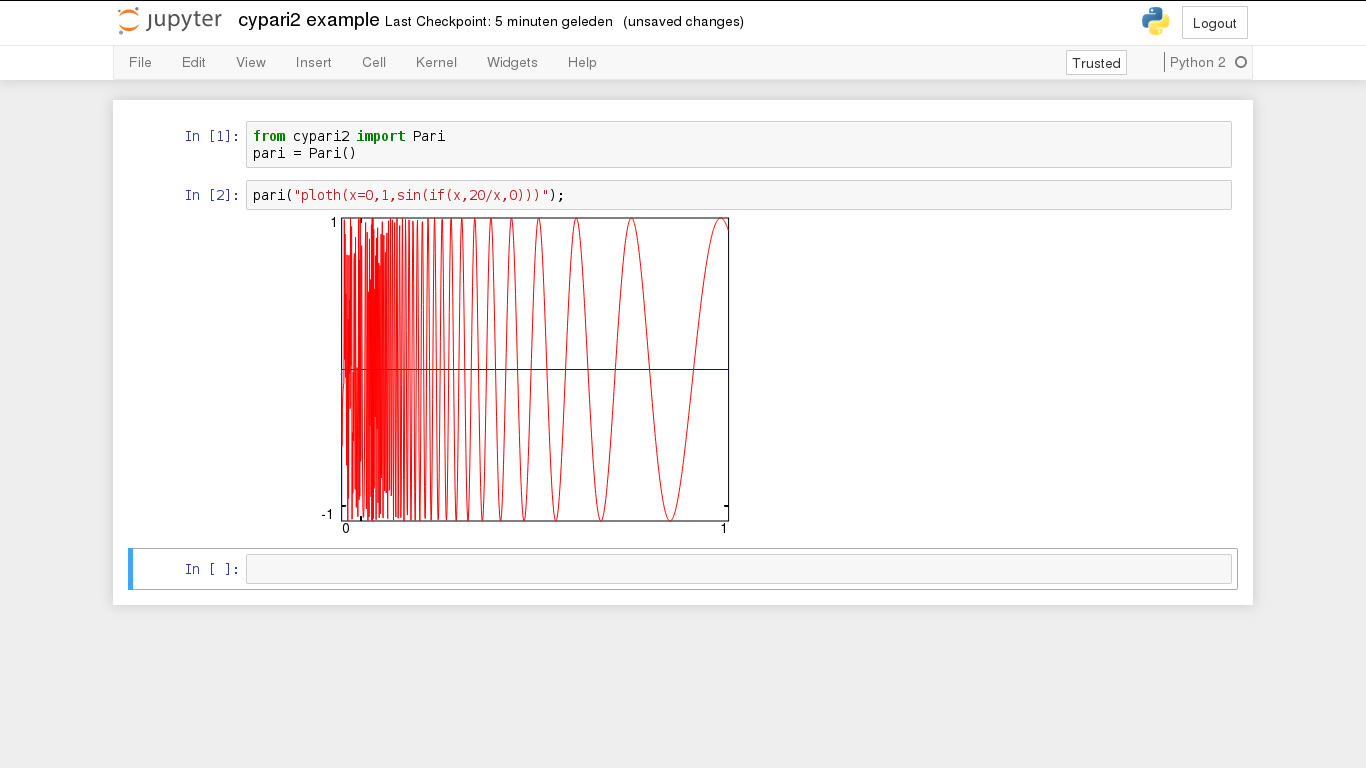
\includegraphics[width=\textwidth,trim={60px 100px 60px 1px},clip]{jupyter-cypari2.png}
  \caption{Plotting using cypari2 in the Python Jupyter kernel}
\end{figure}

\subsection{Support for GP lists}

\TODO{a tiny bit of context to assess how the feature is important;
  e.g. important Pari functions that can now be called; how much
  coverage of the PARI/GP data types do we have now? Was it the last
  piece missing?}

The PARI/GP data type \verb/t_LIST/ is now supported.
This is a dynamic array type, very similar to a Python \verb/list/.

Here, we show how such a list can be used.
We create a list from the vector \verb/[1,2,3]/ and then insert the
element $5$ at the third position:
\begin{verbatim}
>>> from cypari2 import Pari; pari = Pari()
>>> L = pari.List([1,2,3])
>>> L
List([1, 2, 3])
>>> L.listinsert(5, 3)
5
>>> L
List([1, 2, 5, 3])
\end{verbatim}

\subsection{Avoiding copies from the PARI stack}

TODO: Keep objects on the PARI stack instead of always copying

\subsection{Improved auto-generation}

As already reported in \delivref{UI}{pari-python-lib1},
large parts of the cypari2 source code are auto-generated.
Indeed, PARI ships a file \verb/pari.desc/ containing,
for each function, all machine-readable data which is needed to generate
an interface to that function.
This was originally meant to generate a C interface,
but it applies also to a Cython interface.

We have made two improvements to this auto-generation process.
First of all,
the Cython declarations to directly call certain C functions
in the PARI library is now auto-generated.
This is meant to be used by external Cython code
(the original auto-generated code was only for the Python interface)
wanting to interface efficiently with PARI.

\TODO{would you have a quick example illustrating the speed gain of
  calling directly at the Cython level? Maybe mention the number of
  functions auto-generated Cython and Python functions.}

Second, cypari2 now automatically
generates a \texttt{DeprecationWarning}
for obsolete PARI functions.

The following example shows such a deprecation warning
(in Sage since Python does not show such warnings by default),
including the date when the function was deprecated by PARI:
\begin{verbatim}
sage: pari.polred("x^2 + 4")
/usr/local/src/sage-config/src/bin/sage-ipython:1:
DeprecationWarning: the PARI/GP function polred is
obsolete (2013-03-27)
  #!/usr/bin/env sage-python23
[x, x^2 + 1]
\end{verbatim}

\subsection{Documentation}

PARI has a very extensive help for each function.
This help is now translated to docstrings for the Python interface.
This requires a translation from \LaTeX (which is used by PARI)
to reStructuredText (which is used by Sphinx,
the package building the documentation for cypari2).

Since the documentation appears in Cython-generated functions,
we needed a few improvements in Sphinx to make it work
with Cython functions.
This is detailed in the report of \delivref{UI}{sage-sphinx}.
Following standard practice in the Python community,
The built documentation is now also available on the
documentation hosting service ReadTheDocs;
see \url{https://cypari2.readthedocs.io/}.

\subsection{Compatibility improvements}

\TODO{The intro of D4.1 on
  https://github.com/OpenDreamKit/OpenDreamKit/issues/83 states: “The
  CyPari2 package is not ready to replace the PyPi package CyPari yet.
  The most important missing functionality is Windows compatibility. A
  full replacement to CyPari is the goal of deliverable D4.10.”.
  Please elaborate briefly on that here.}

\TODO{The title of this section could be something like ``CyPari2 as a
  standalone Python package''}

\TODO{State a few words about the adoption of CyPari2; e.g. is it used
  by Snappy?}

The primary motivation of the cypari2 package
was to be used as part of the Sage distribution.
However, we want it to be usable also by itself, outside of Sage.
We made several improvements to make that possible:
the code is now fully compatible with Python 3 (starting with with version 3.4)
and with multiple versions of PARI (from 2.9.0 to the most recent release, 2.11.0).
To ensure that it remains compatible, multiple Python and PARI
versions are tested on the continuous integration platform Travis CI.


\TODO{The intro of D4.1 says: ``Because of the high degree of
  coupling, and thanks to the availability of Snappy, this deliverable
  constitutes a highly valuable case study for future externalizations
  of low-level interfaces in SageMath.''; a few words about the lesson
  learned while treating this use case would be interesting. Also
  mention the latest workshop in Cernay where you reported on that
  experience.}

\end{document}
